\documentclass[12pt,tikz]{standalone}
\pdfinfoomitdate 1
\pdfsuppressptexinfo 1
\pdftrailerid{}
\usepackage[utf8]{inputenc}
\usepackage{amsmath}
\usepackage{pgfplots}
\usepackage{tikz}
\usetikzlibrary{shapes.geometric}
\pagestyle{empty}

\begin{document}
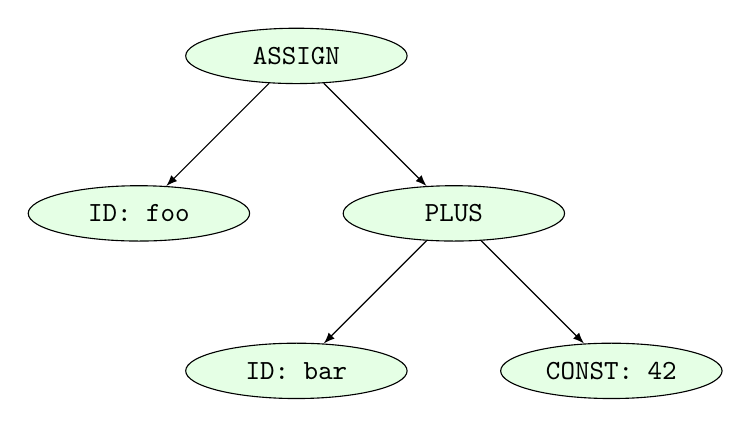
\begin{tikzpicture}
	\tikzstyle{node} = [draw, fill=green!10, ellipse, minimum height=2em, minimum width=8em, node distance=10em]

	\draw (+0,+0) node[node] (n1) {\tt ASSIGN};

	\draw (-2,-2) node[node] (n11) {\tt ID: foo};
	\draw (+2,-2) node[node] (n12) {\tt PLUS};

	\draw (+0,-4) node[node] (n121) {\tt ID: bar};
	\draw (+4,-4) node[node] (n122) {\tt CONST: 42};

	\draw[-latex] (n1) -- (n11);
	\draw[-latex] (n1) -- (n12);

	\draw[-latex] (n12) -- (n121);
	\draw[-latex] (n12) -- (n122);
\end{tikzpicture}
\end{document}
